\section{Client Usage}
\label{sec:client_usage}
The client can generally do three things; commit a problem, see status of his/her problems, or search the database for problems.
The first two are based on there corresponding use cases in section \ref{sec:usecase}.
The search function was added as a functionality for client because we assume that it would primarily be persons with a new problem who might want to search for others problems.

The following subsections describes the three usage of the system which the \aclient[] has access to.

\subsection{Commit a Problem}
When a client wants to commit a problem he/she is asked to categorize the problem in the window showed in figure \ref{fig:commit}

\begin{figure}
	\centering
		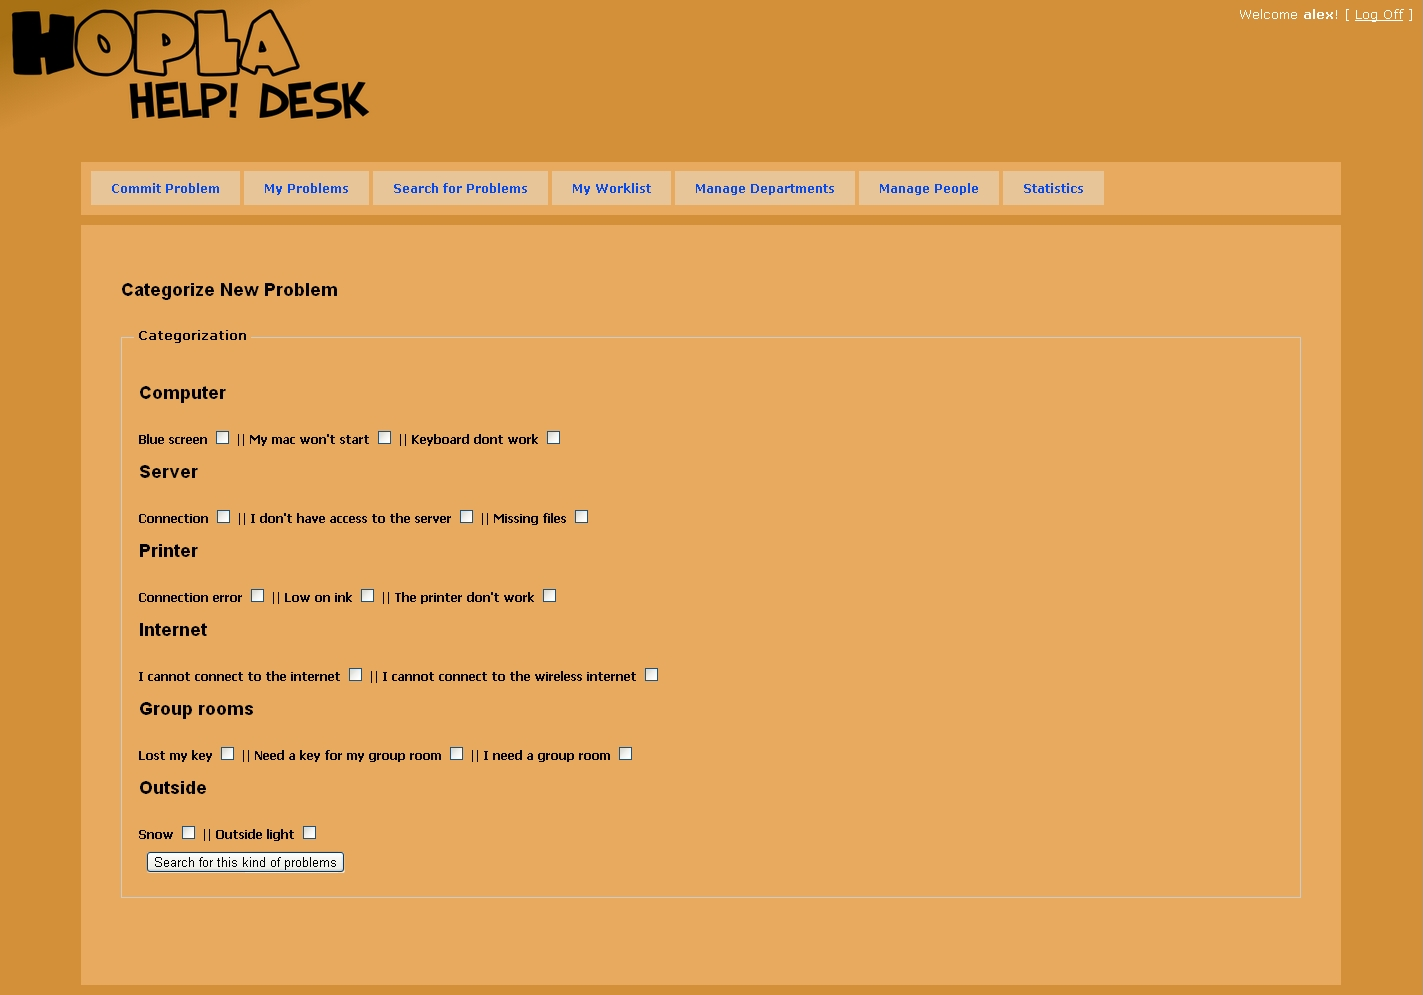
\includegraphics[width=1.00\textwidth, clip=true, trim=2.9cm 0.5cm 3cm 8cm]{input/implementation/program_presentation/commit.png}
	\caption{The categorization step in commiting a problem}
	\label{fig:commit}
\end{figure}


\subsection{See Own Problems}


\subsection{Search for Problems}